\documentclass[12pt,oneside,a4paper,parskip]{scrbook}
\usepackage[utf8]{inputenc}
\usepackage{csquotes}
\usepackage[ngerman]{babel}
\usepackage{floatflt}
\usepackage{subfigure}
\usepackage[pdftex]{graphicx}
\usepackage[hidelinks]{hyperref}
\usepackage{color}
\usepackage{amssymb}
\usepackage{textcomp}
\usepackage{nicefrac}
\usepackage{scrhack}
\usepackage{pdfpages}
\usepackage{float}
\usepackage{pdflscape}
\usepackage{subfigure}
\usepackage{pdfpages}
\usepackage[verbose]{placeins}
%\usepackage[nouppercase,headsepline,plainfootsepline]{scrpage2}
\usepackage{listings}
\usepackage{xcolor}
\usepackage{color}
\usepackage{caption}
\usepackage{subfigure}
\usepackage{epstopdf}
\usepackage{longtable}
\usepackage{setspace}
\usepackage{booktabs}
\usepackage[style=numeric,backend=biber, uniquelist=false]{biblatex}
\bibliography{literatur}
\addbibresource{literatur.bib}


%%%%%%%%%%%%%%%%%%%
%% definitions
%%%%%%%%%%%%%%%%%%%
\def\BaAuthor{David Mödl\, Sebastian Lober}
\def\BaAuthorStudyProgram{Informatik} %% Wirtschaftsinformatik, E-Commerce, Informationssysteme
\def\BaType{Seminararbeit} %% Masterarbeit
\def\BaTitle{Bias of Neural Networks - Security implications}
\def\BaSupervisorOne{Prof.\ Dr.\ A B}
\def\BaSupervisorTwo{Prof.\ Dr.\ C D}
\def\BaDeadline{\today}

\ifdefined\iswithfullname
  \def\ShowBaAuthor{\BaAuthor}
\else
  \def\ShowBaAuthor{N.~N.}
\fi

\hypersetup{
pdfauthor={\ShowBaAuthor},
pdftitle={\BaTitle},
pdfsubject={Subject},
pdfkeywords={Keywords}
}

%%%%%%%%%%%%%%%%%%%
%% configs to include
%%%%%%%%%%%%%%%%%%%
\colorlet{punct}{red!60!black}
\definecolor{background}{HTML}{EEEEEE}
\definecolor{delim}{RGB}{20,105,176}
\colorlet{numb}{magenta!60!black}

\definecolor{gray}{rgb}{0.4,0.4,0.4}
\definecolor{darkblue}{rgb}{0.0,0.0,0.6}
\definecolor{cyan}{rgb}{0.0,0.6,0.6}

\definecolor{pblue}{rgb}{0.13,0.13,1}
\definecolor{pgreen}{rgb}{0,0.5,0}
\definecolor{pred}{rgb}{0.9,0,0}
\definecolor{pgrey}{rgb}{0.46,0.45,0.48}

\lstset{
  basicstyle=\ttfamily,
  columns=fullflexible,
  showstringspaces=false,
  commentstyle=\color{gray}\upshape
  linewidth=\textwidth
}

\lstdefinelanguage{json}{
    basicstyle=\normalfont\ttfamily,
    numbers=left,
    numberstyle=\scriptsize,
    stepnumber=1,
    numbersep=8pt,
    showstringspaces=false,
    breaklines=true,
    backgroundcolor=\color{background},
    literate=
     *{0}{{{\color{numb}0}}}{1}
      {1}{{{\color{numb}1}}}{1}
      {2}{{{\color{numb}2}}}{1}
      {3}{{{\color{numb}3}}}{1}
      {4}{{{\color{numb}4}}}{1}
      {5}{{{\color{numb}5}}}{1}
      {6}{{{\color{numb}6}}}{1}
      {7}{{{\color{numb}7}}}{1}
      {8}{{{\color{numb}8}}}{1}
      {9}{{{\color{numb}9}}}{1}
      {:}{{{\color{punct}{:}}}}{1}
      {,}{{{\color{punct}{,}}}}{1}
      {\{}{{{\color{delim}{\{}}}}{1}
      {\}}{{{\color{delim}{\}}}}}{1}
      {[}{{{\color{delim}{[}}}}{1}
      {]}{{{\color{delim}{]}}}}{1},
}

\lstset{language=xml,
  morestring=[b]",
  morestring=[s]{>}{<},
  morecomment=[s]{<?}{?>},
  stringstyle=\color{black},
  numbers=left,
  numberstyle=\scriptsize,
  stepnumber=1,
  numbersep=8pt,
  identifierstyle=\color{darkblue},
  keywordstyle=\color{cyan},
  backgroundcolor=\color{background},
  morekeywords={xmlns,version,type}% list your attributes here
}

\lstset{language=Java,
  showspaces=false,
  showtabs=false,
  tabsize=4,
  breaklines=true,
  keepspaces=true,
  numbers=left,
  numberstyle=\scriptsize,
  stepnumber=1,
  numbersep=8pt,
  showstringspaces=false,
  breakatwhitespace=true,
  commentstyle=\color{pgreen},
  keywordstyle=\color{pblue},
  stringstyle=\color{pred},
  basicstyle=\ttfamily,
  backgroundcolor=\color{background},
%  moredelim=[il][\textcolor{pgrey}]{$$},
%  moredelim=[is][\textcolor{pgrey}]{\%\%}{\%\%}
}

\newcommand*{\forcetwosidetitle}[1][1]{%
 \begingroup
   \cleardoubleoddpage
   \KOMAoptions{titlepage=true}% useful e.g. for scrartcl
   \csname @twosidetrue\endcsname
   \maketitle[{#1}]
 \endgroup
}


\begin{document}


%%%%%%%%%%%%%%%%%%%
%% Titelseite
%%%%%%%%%%%%%%%%%%%


\frontmatter
\titlehead{%  {\centering Seitenkopf}
  {Hochschule für angewandte Wissenschaften Würzburg-Schweinfurt\\
   Fakultät Informatik und Wirtschaftsinformatik}}
\subject{\BaType}
\title{\BaTitle\\[15mm]}
%\subtitle{\normalsize{vorgelegt an der Hochschule f\"{u}r angewandte Wissenschaften W\"{u}rzburg-Schweinfurt in der Fakult\"{a}t Informatik und Wirtschaftsinformatik zum Abschluss eines Studiums im Studiengang \BaAuthorStudyProgram}}
\author{David Mödl \& Sebastian Lober}
%\date{\normalsize{Eingereicht am: \BaDeadline}}
%\publishers{
%  \normalsize{Erstpr\"{u}fer: \BaSupervisorOne}\\
%  \normalsize{Zweitpr\"{u}fer: \BaSupervisorTwo}\\
%}
\forcetwosidetitle


%%%%%%%%%%%%%%%%%%%
%% abstract
%%%%%%%%%%%%%%%%%%%

\section*{Zusammenfassung}

TODO

\section*{Abstract}
KI steht kurz für künstliche Intelligenz. Der Begriff KI ist jedoch irreführend. Eine 'KI' ist ein Programm, das versucht biologisches intelligentes Verhalten nachzuahmen. Die Begrifflichkeit Intelligenz in Verbindung mit Computern ist sehr umstritten, dennoch wird im Allgemeinen als auch in der Forschung das Wort 'Intelligenz' verwendet. \\
Aus diesem Grund und an Mangel an qualitativ hochwertigen Alternativen wird auch im Folgenden der Wortlaut KI verwendet, wohl wissend, dass die Bezeichnung nicht 100 Prozent korrekt ist.

%%%%%%%%%%%%%%%%%%%
%% Inhaltsverzeichnis
%%%%%%%%%%%%%%%%%%%
\tableofcontents



%%%%%%%%%%%%%%%%%%%
%% Main part of the thesis
%%%%%%%%%%%%%%%%%%%
\mainmatter

\chapter{Einführung}
\label{chapter:intro}
Künstliche Intelligenz(KI) oder auch artifizielle Intelligenz(AI) tritt allgegenwärtig in großen Teilen unserer Gesellschaft auf. Von Kaufvorschlägen auf Amazon, über Chat-Bots bis hin zu autonom fahrenden Autos spielt die KI eine große Rolle. Ein bekanntes Beispiel ist die Software "alpha go", welche den internationalen GO Champion Lee Sedol besiegte\cite{alphaGo}. Darüber hinaus ermöglicht die KI komplexe Sachverhalte zu simulieren und zu prognostizieren, wie zum Beispiel die vollautomatische Generierung hochaufgelöster, realistischer Videosequenzen auf der Grundlage simpler Eingaben\cite{videoToVideo}.
\\\\
Einerseits gibt es viele Erfolge, die für ein KI betriebenes System sprechen. Andererseits bestärken medienwirksame Verfehlungen, wie z.B. das frauenfeindliche Bewerbungssystem von Amazon\cite{amazon}, die Skeptiker solcher Systeme. Ziel dieser Arbeit ist es, die unterschiedlichen Ursprünge solcher algorithmischen Verzerrungen (engl. bias) zu erläutern und Präventionen zu schildern, welche diese vermeiden sollen.
\\\\
Wir beginnen unsere Arbeit damit, Grundlagen für ein fundamentales Wissen spätere Kapitel aufzubauen. Danach möchten wir auf die Entstehung solcher Bias eingehen, die damit verbundenen Probleme und welche Präventionen gegen diese Fehlverhalten unternommen werden können.
\chapter{Grundlagen}
\section{Bias}
Wesentlicher Bestandteil der Arbeit ist das erläutern der "Biases", welche durch die Nutzung von künstlicher Intelligenz auftreten können. Das Wort Bias kommt aus dem Englischen und bedeutet im Wesentlichen:

\begin{enumerate}
	\item Verzerrung – im statistischen Sinn als mittlere systematische Abweichung zwischen dem erwarteten („richtigen“) Modellergebnis und dem mittleren wirklich eingetretenen Modellergebnis.
	\item Voreingenommenheit – je nachdem, wie wir die Welt aufgrund unserer Erfahrungen sehen, kommen wir zu unterschiedlichen Schlüssen.
\end{enumerate}

Der Begriff Voreingenommenheit muss bei der Nutzung von KI vorsichtig behandelt werden, denn eine Maschine besitzt grundsätzlich keinerlei Vorurteile und weiß zu Beginn nicht was richtig oder falsch ist. Hier spricht man daher von einem Fehlverhalten oder einer Verzerrung, welche durch äußere Einflüsse wie z.B. dem Menschen verursacht wurden.\\

\section{Künstliche Intelligenz}
Künstliche Intelligenz (KI) oder englisch artificial intelligence (AI) ist der Oberbegriff für ein Teilgebiet der Informatik. Dieses Gebiet befasst sich nicht nur mit neuronalen Netzen, sondern generell mit jeglicher Form von maschinellen intelligenten Verhalten und dem maschinellen Lernen, siehe Abbildung \ref{fig:Uebersicht}. Generell wird bei der künstlichen Intelligenz versucht biologische Intelligenz auf einen Computer zu simulieren. Dies basiert meist auf simplen Algorithmen, wodurch die Begrifflichkeit 'Intelligenz' in Bezug auf Maschinen öfter in Frage gestellt wird.
% Oder hier irgenwas zitieren hier.
% Das Rad muss nicht immer neu erfunden werden.

\begin{figure}[ht]
	\begin{center}
		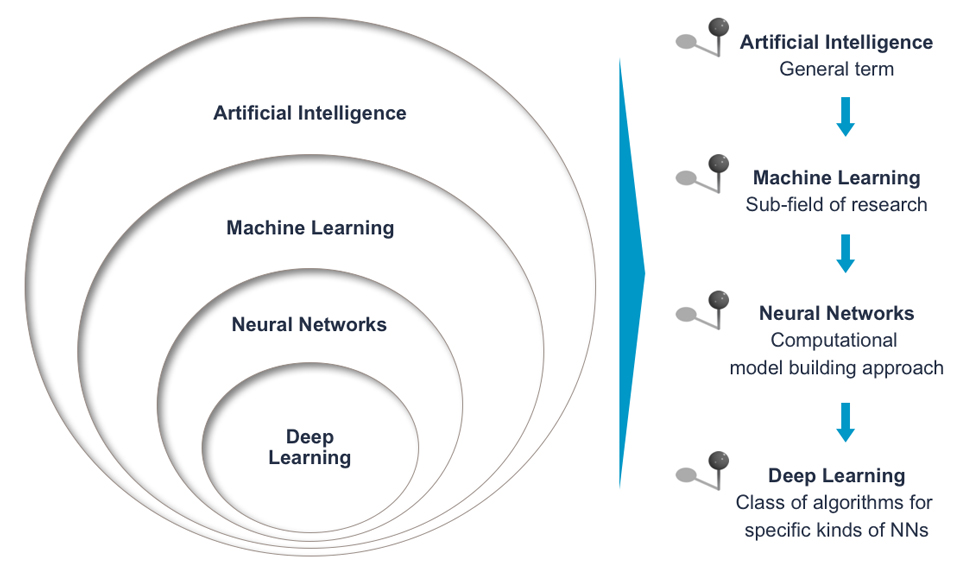
\includegraphics[width=14cm]{Bilder/Abstraktionslevel_von_AI.jpg}
		\caption{Verschiedene Abstraktionslevel von Artificial Intelligence in hierarchischer Ordnung}
		\label{fig:Uebersicht}
	\end{center}
\end{figure}
%https://www.capgemini.com/de-de/2017/09/artifical-intelligence-machine-learning-und-data-science-same-same-but-different/
Damit ein Programm den Titel KI tragen darf, muss sie zum einen die Fähigkeit zu lernen besitzen, zum anderen die Fähigkeit auch bei nicht eindeutigen Eingaben intelligent Lösungen zu finden.\\
KIs werden grob in zwei Kategorien aufgeteilt.
Die starke KI besitzt eine Intelligenz, die dem eines Menschens eben würdig ist bzw. sogar übersteigt. Ob eine starke KI überhaupt jemals erreicht wird, ist sehr umstritten. \\Schwache KI hingegen sind in unserem Alltag bereits vertreten. Schwache KI sind Algorithmen, die ganz spezielle Aufgaben lösen und die Arbeit von Menschen unterstützen.
% symbolische vs. neuronale KI
% Simulationsmethode vs. phänomenologische Methode
% Problemlösungsansätze: Suchen, Planen, Optimieren, logisches Schließen, Approximieren
\subsection{Maschine Learning}
Machine Learning (ML) ist ein Teilgebiet der künstlichen Intelligenz. Es ist der Oberbegriff jeglicher Lernvarianten von KIs. Im Allgemeinen versucht eine KI neue Muster und Gesetzmäßigkeiten in Trainingsdaten zu erkennen, diese zu verallgemeinern und für neue Problemlösungen oder für die Analyse von bisher unbekannten Daten zu verwenden\cite{EliminateHumanBias}.
\\\\Diese Arbeit speziell konzentriert sich auf Deep Learning, welches eine Variante zum Trainieren von neuronalen Netzen darstellt.
\subsubsection{Lernformen}
KIs bestehen aus vielen Algorithmen. Damit eine KI lernt, müssen diese Algorithmen angepasst werden. Hierbei gibt es drei übergeordnete Lernformen: überwachtes, unüberwachtes oder bestärkendes Lernen. \\\\
Beim überwachten Lernen sind Trainingsdaten bereits kategorisiert. Nach dem Versuch die Daten eigenständig zu kategorisieren, erhält das KI-System ein positives oder negatives Feedback. Auf Basis des Feedbacks lernt die KI, auf welche Muster und Merkmale es achten muss, um die Aufgabe richtig zu lösen. \\
Die andere Variante ist das unüberwachte Lernen. Hierbei sind die Trainingsdaten nicht kategorisiert und das KI-System kann somit kein Feedback bekommen. Das neuronale Netz erstellt ein statisches Model aus den Trainingsdaten und versucht Zusammenhänge und wiederkehrende Muster zwischen den Daten zu erkennen. Zusammenhängende Daten werden einer Kategorie zugeordnet. Die lernende KI weiß zu keiner Zeit, ob das was es Gruppiert auch zusammengehört.\\
Bestärkendes Lernen (auch Reinforcement Learning) ist eine Lernmethode bei dem der Algorithmus durch Belohnung und Bestrafung trainiert wird. Verstärkungslernen wird zum Beispiel beim Trainieren von Spielen angewandt. Hierbei erhält das KI-System Feedback in Form von Belohnung, wenn sein Verhalten zum Sieg geführt hat oder eine Bestrafung, falls das bestimmte Verhalten nicht zielführend war. Mit dieser Lernmethode wurde Google AlphaGo trainiert, die als erstes Computer Programm 2016 den weltbesten Profispieler im komplexen Brettspiel Go besiegen konnte.
\subsection{Neuronale Netze}
Künstliche neuronale Netze (KNN) bestehen aus künstlichen Neuronen, die untereinander verflechtet sind. Diese Konstrukte sind denen der sich im Nervensystem eines Lebewesens befindenden Neuronenverbindungen nachempfunden. \\
KNNs sind nicht dazu da das Nervensystem von Lebewesen nachzubilden, sondern abstrakt die Eigenschaften der Informationsverarbeitung und der Lernfähigkeit zu imitieren.
\begin{figure}[h]
	\begin{center}
		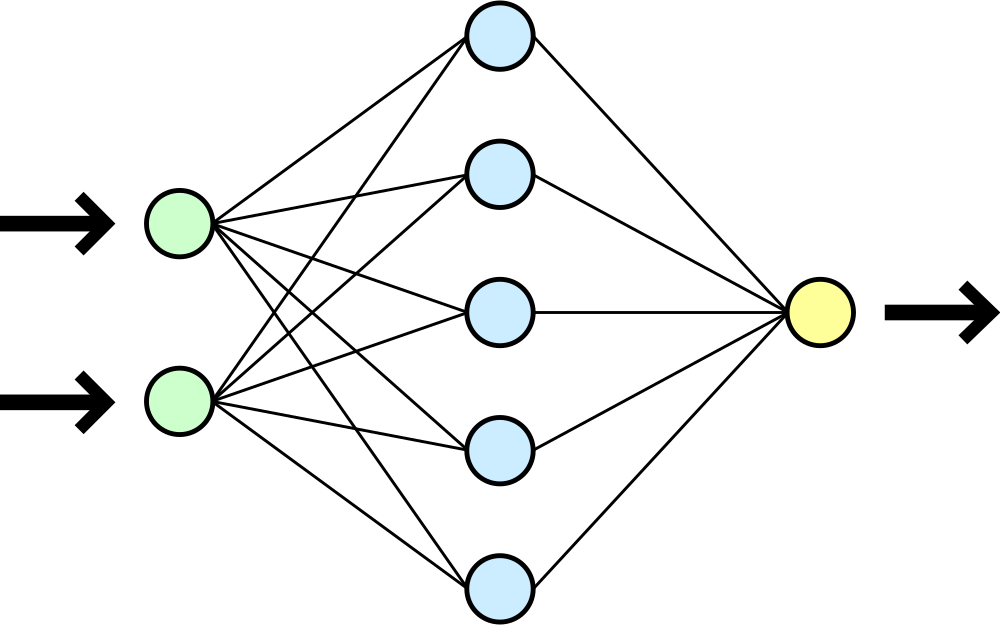
\includegraphics[width=12cm]{Bilder/Neurales_Netz.png}
		\caption{Vereinfachte Darstellung eines künstlichen neuronalen Netzes}
		\label{fig:wikiNeuronalesNetz}
	\end{center}
\end{figure}
% https://de.wikipedia.org/wiki/K%C3%BCnstliches_Neuron#/media/Datei:ArtificialNeuronModel_deutsch.png
KNNs sind meist in Schichten mit beliebig vielen künstlichen Neuronen aufgebaut. In der Regel besteht ein KNN aus drei Teilen die Eingangsschicht (grün), verdeckte Schicht (blau) im Englischen Hidden Layer und die Ausgabeschicht (gelb). In der Eingangsschicht fließen die Informationen in das Netz ein und in der Ausgabeschicht das Ergebnis der Berechnungen aus. Jede Schicht besteht aus beliebig vielen Neuronen je nach Komplexität des Zieles, die Hidden Layer sogar aus beliebig viele Schichten.
\\\\
In der Regel arbeiten KNNs nach dem feedforward-Prinzip, bei dem die Informationen nur in eine Richtung fließen. Es gibt jedoch auch rekurrente Netze, bei denen durch rückgerichtete Kanten Rückkopplungen im Netz entstehen. \\
Die einfachste Netzstruktur ist das einschichtige feedforward-Netz. Dies besteht ohne Rückkopplungen aus nur einer Schicht, der Ausgabeschicht.
\subsubsection{Das künstliche Neuron}
Künstliche Neuronen sind die Grundbestandteile eines künstlichen neuronalen Netzes.
Ein künstliches Neuron ist die vereinfachte und abstrakte Version einer biologischen Nervenzelle und ist wie folgt aufgebaut.\\\\
\begin{figure}[h]
	\begin{center}
		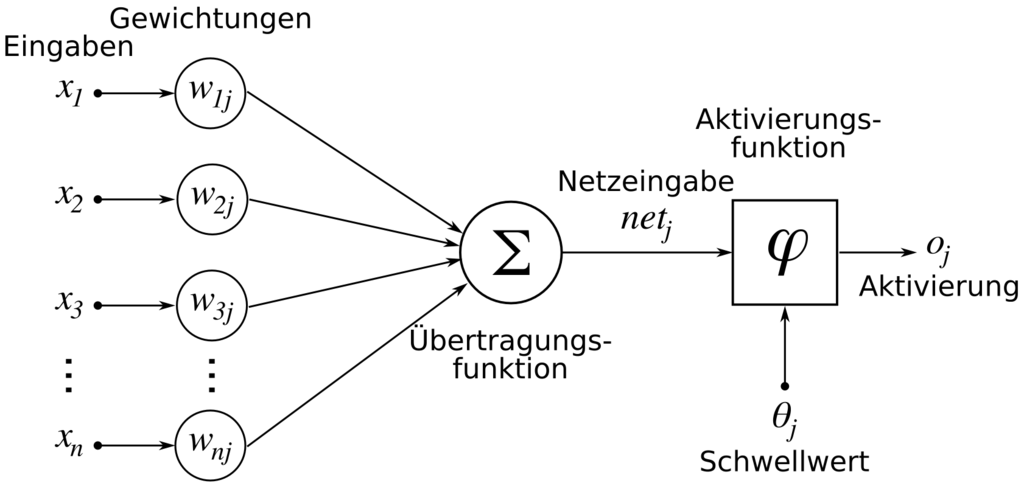
\includegraphics[width=12cm]{Bilder/ArtificialNeuronModel_deutsch.png}
		\caption{Ein künstliches Neuron}
		\label{fig:wikiNeuron}
	\end{center}
\end{figure}
% https://de.wikipedia.org/wiki/K%C3%BCnstliches_Neuron#/media/Datei:ArtificialNeuronModel_deutsch.png
Ein künstliches Neuron besitzt $n$ Eingangskanäle und einen Ausgangskanal. $j$ repräsentiert hier die eindeutige Nummer des Neuron. Jede Eingabe $x_{i}$ besitzt ein dazugehörendes Gewicht $w_{1j}..w_{nj}$. Dieser spiegelt die Wichtigkeit der Eingabe wider, diese kann hemmend negativer oder erregend positiver Wert wirken. Die Übertragungsfunktion $\Sigma$ summiert alle multiplizierten Eingaben mit ihrem Gewicht und geht als Netzeingabe $net_j$ in die Aktivierungsfunktion $\varphi$ ein. \\
Ob das Neuron "'feuert"' oder kein Signal sendet, wird hier berechnet. Auf die Netzeingabe $net_j$ wird ein Schwellenwert $\theta_j$ addiert. Als mathematisch Vereinfachung wird der Schwellwert $\theta$ als $w_0$ bezeichnet und $x_0 = 1$ eingeführt und somit in der folgenden Formel immer auf die Netzeingabe $net_j$ addiert.
\\\\
${\displaystyle a=\sum _{i=0}^{n}x_{i}w_{i}}$
\\\\
Die Variabel $a$ geht in die Aktivierungsfunktion ${\sigma (a)}$ ein, anhängig von dem Ergebnis wird das Neuron aktiv oder bleibt inaktiv.
Der Ausgangskanal eines Neuron ist gleichzeitig ein Eingangskanal eines oder mehreren anderen Neuronen. % Den Satz nochmal überprüfen
\\\\
Dadurch dass ein Neuron mehrere Eingangskanäle besitzt, werden viele Eingangsinformationen auf ein Ergebnis reduziert. Durch mehrere Schichten und vielen Neuronen pro Schicht kann so eine große Menge an Daten schnell reduziert werden.
\\\\
Jedoch muss jedes künstliche Neuron eines KNNs richtig eingestellt werden, damit das KNN dessen Ziel erfüllt. Eingestellt wird das Neuron durch Training. Trainieren bedeutet hier das Ermitteln der richtigen Werte für Gewichtungen und Schwellwerte, als auch das Einstellen der richtige Verbindungskombinationen der Neuronen untereinander. Diesen Prozess nennt man Deep Learning, eine Form von Machine Learning.
\subsection{Deep Learning}
Deep Learning ist eine Maschine Learning Variante, die speziell bei künstliche neuronale Netze eingesetzt wird. Beim Deep Learning werden die zahlreichen Zwischenschichten der Hidden Layer trainiert. Dabei wird eine umfangreiche und komplexe Struktur der Neuronen-Verbindungen aufgebaut. Wie das Programm endgültig die Aufgabe lösen soll, wird hierbei nicht vorgegeben, sondern bei diesem autonomen Prozess evolutionär ermittelt.
\\\\
Ein künstliches neuronales Netz wird mit dem Zweck aufgebaut, eine bestimmte Aufgabe zu lösen. Extra dafür müssen Trainingsdaten aufbereitet werden. Diese Art der Daten, beispielsweise Bilder, soll das fertig trainierte Netz richtig interpretieren können. Trainings und Testdaten sind Daten, bei dem das korrekte Ergebnis bekannt ist.
\\\\
Am Anfang ist das künstliche neuronale Netz meist mit relativ zufälligen Werten und Verbindungen vorbelegt. Trainingsdaten werden dem zu trainierenden Netzwerk an die Eingangsschicht übergeben. Diese durchlaufen das Netz. Das Ergebnis wird an der Ausgabeschicht überprüft. Die Ausgabeschicht besteht im einfachsten Fall aus zwei Neuronen, beispielsweise "'Gesicht erkannt"' oder "'kein Gesicht"', an dem gemessen wird, wie viel gewichtete Signale ankommen. Diese summiert, ergeben die Endergebnisse der Berechnungen und das Neuron mit dem höchsten Gewicht, ergibt die Antwort.
\\\\
Neuronale Netze sind für Menschen ab einer gewissen Größe nicht mehr nachvollziehbar. Somit kann nur die Eingabe mit der Ausgabe mit Hilfe von Testdaten verglichen werden, um auf die Korrektheit der Aufgabenlösung zu prüfen. Ziel ist es mit möglichst vollständigen Trainingsdaten das Netzwerk so einzustellen, dass diese nicht nur die Trainingsdaten und Testdaten richtig beantwortet, sondern auch unbekannt Daten korrekt interpretiert.
\\\\
Um eine Aufgabe, wie ''Gesicht in Bild erkennen'', zu trainieren, wird nicht nur ein Netz mit Zufallswerten und Verbindungen generiert sondern tausende. Alle werden mit den gleichen Testdaten geprüft und für jedes Netz ein Mittelwert über die Korrektheit der Antworten erstellt. Da alle Netze Initial mit Zufallswerten belegt sind, haben die meisten Netze eine Erfolgsrate von ca. 50 Prozent. Die Netze mit den höchsten Erfolgsraten, mit beispielsweise mehr als 60 Prozent, werden behalten, der Rest wird verworfen. Die erfolgreichsten Netze werden mehrfach kopiert und bei jedem Kopiervorgang individuell leicht verändert und erneut getestet. Die Besten werden wieder genommen und leicht modifiziert kopiert und schlechteren verworfen.
\\\\
Nach einer gewissen Anzahl an Iterationen entscheidet das Netz nicht mehr willkürlich, sondern scheint intelligent die Aufgabe zu lösen. Dieser Iterationsschritt kann unendlich oft laufen, jedoch empfiehl es sich, je nach Anwendungsfall, ab einer gewissen Erfolgsrate das Training zu beenden oder neue Trainings- und Testdaten zu verwenden. Als Ergebnis des Prozesses erhält man durch Deep Learning ein trainiertes künstliches neuronales Netz, das im Allgemeinen als KI bezeichnet wird.

\subsection{Loss-Funktion}
\label{section:lossFunction}

Alle Modelle benötigen eine Loss-Funktion(Verlustfunktion), um später trainiert werden zu können. Die Verlustfunktion bestimmt die Differenz zwischen der Prognose, die das Modell liefert, und dem vorgegebenen Label. Sie muss für die Menge aller Daten berechnet werden und beschreibt damit, wie gut das Modell die Trainingsdaten abbildet.
% vll noch Beispiel dazu
%https://www.ai-united.de/arbeitsweise-eines-neuronalen-netzwerkes-algorithmen-training-aktivierungs-und-verlustfunktionen/
%https://www.sigs-datacom.de/trendletter/2018-06/12-werkzeugneutrale-einfuehrung-in-maschinelles-lernen.html

\section{Daten}
\label{section:Data}
Erst durch eine Kombination aus Algorithmen und Daten wird die Entscheidungsfindung unterstützt. Wie ein menschlicher Entscheider können auch Algorithmen wegen unvollständiger oder fehlerhafter Daten zu fehlerhaften Entscheidungen gelangen. Eine gute Datenqualität und viele Daten ist daher unabdingbar. Auch die richtige Unterteilung zwischen Test- und Trainingsdaten spielt darf bei maschinelles Lernen nicht vergessen werden.

\subsection{Datenaufbereitung}
\label{section:dataSetup}
Der Erfolg einer KI hängt von den Daten ab mit welchen dieses Modell trainiert und getestet wird. Zuerst müssen Daten gesammelt werden, welche zu dem Zweck der KI passen. Soll eine System Äpfel und Birnen unterscheiden, müssen Bilder gesammelt werden, welche Birnen und Äpfel enthalten.
\\\\
Um nun ein Modell trainieren zu können, müssen die Daten in Trainings- und Testdaten unterteilt werden. Die Testdaten werden nicht für das Training benutzt, sondern dienen dazu, das fertige System gegen unbekannte Daten zu testen, mit welchen es zuvor nicht trainiert wurde. Meist werden 10-20\% der Daten als Testdaten reserviert. Die Trainingsdaten werden genutzt um das Modell zu trainieren.
\\\\
Bei überwachtem Lernen müssen die Daten zuvor ein Label enthalten, welches der KI mitteilt um was es sich bei diesem Datensatz handelt, z.B. muss ein Birne auch als solche gekennzeichnet werden.
\\\\
Ein Datensatz besteht grundsätzlich aus 2 Elementen. Beim überwachten Lernen wird wie bereits genannt, das Label welches man Vorhersagen möchte, benötigt. Anhand unseres Beispiels wäre ein Attribut welches dem Programm sagt, ob es sich auf dem Bild um eine Birne oder einen Apfel handelt. Damit die Maschine leichter Muster erkennen kann, werden dazu weitere Eigenschaften (z.B. Farbe, Größe) benötigt. Diese helfen dem Modell z.B. das Label richtig vorherzusagen.

\subsection{Quantität}
\label{section:DataQuantity}
Je mehr unterschiedliche Eigenschaften in den Datensätzen existieren, umso komplexer wird das Modell. Und diese Komplexität der Probleme erfordert, dass die Menge an Daten entsprechend groß sein muss, damit das zu trainierende System, alle Algorithmen korrekt einstellt.
\\\\
Ein Beispiel hierfür findet sich in der Autoindustrie. Beim autonomen Fahren müssen Daten von Laser-, Kamera- und Radarsensoren im Auto zuverlässig und schnell verarbeitet werden. Die KI im Fahrzeug muss jederzeit über ein präzises Abbild der realen Verkehrsbedingungen verfügen, um darauf basierend in jeder Fahrsituation die richtige Entscheidung treffen zu können \cite{autonomesFahren}.
\\\\
Je nach Komplexität der Anwendungen werden mehr oder weniger Datensätze benötigt. Generell kann man sagen, dass mit zu wenigen Trainingsdaten, ein KNN schwerer Muster in den Daten erkennt und dadurch fehleranfälliger wird.

%Anhand dieses Beispiels erkennt man die Wichtigkeit der Quantität der Trainingsdaten, da die Anzahl möglicher Situationen im Straßenverkehr prinzipiell unendlich ist. Um gleichartige Strukturen im Verkehrsgeschehen zu erkennen, sind viele Trainingsdaten erforderlich, die ein immer genaueres Bild ergeben.

\subsection{Qualität}
\label{section:DataQuality}

Die Qualität der Daten ist für maschinelles Lernen essentiell. Eine hohe Datenqualität wird erreicht, indem man Widersprüchlichkeiten innerhalb der Datenbeständen vermeidet, die Interpretierbarkeit der Daten gewährleistet, die Manipulationsgefahr der Daten verhindert und die Integrität dieser sicherstellt\cite{dataQuality}.
Um das umsetzen zu können wird ein Zugang zu den Daten benötigt, damit diese kontrolliert und angepasst werden können.\\
Beim überwachten Lernen wird zudem wie bereits in Absatz \ref{section:dataSetup} beschrieben, ein korrektes Label gebraucht. Sind Daten nicht vollständig und fehlen bestimmte Anwendungsfälle, ethische Gruppe, Geschlechter, kann die KI diese in der Praxis nicht korrekt beantworten, siehe Abschnitt \ref{section:uncompleteData}.
% https://qymatix.de/de/predictive-analytics-methoden-datenqualitaet/

\chapter{Bias Entstehung}
Bei der Nutzung von KI System können Verzerrungen(Bias) bzw. Fehlverhalten entstehen, diese können unterschiedlicher Natur sein und an unterschiedlichen Stellen, in der in Abbildung \ref{fig:dataBias} gezeigten, vereinfachten Machine Learning Pipeline, auftreten. Dabei möchten wir auf die Daten eingehen, welche bei der Eingabe zu Bias führen können und menschliche Fehler verdeutlichen, welche bei der Verarbeitung und der Ausgabe auftreten können. Zuletzt möchten wir Adversial Attacks ansprechen, welche zu weiteren Verzerrungen führen können.

\begin{figure}[h]
	\begin{center}
		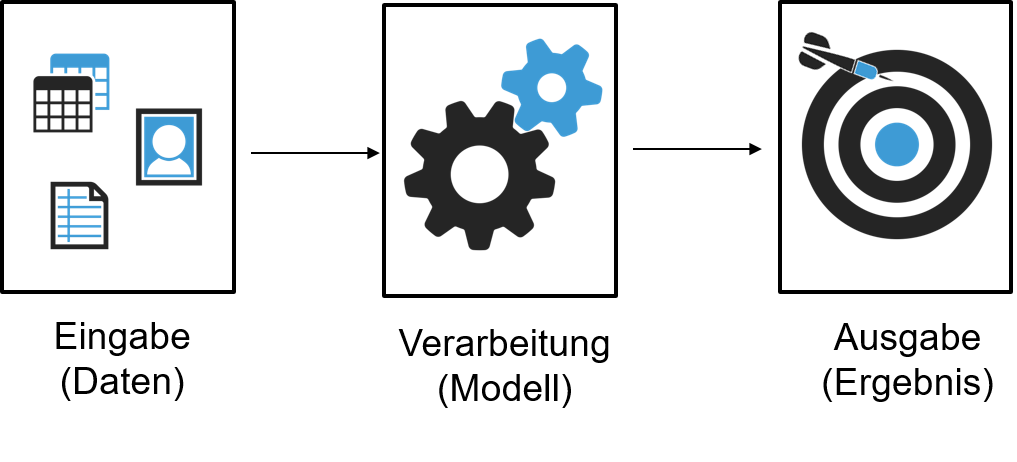
\includegraphics[width=12cm]{Bilder/data_bias.png}
		\caption{Machine Learning Pipeline: Eingabe, Verarbeitung, Ausgabe}
		\label{fig:dataBias}
	\end{center}
\end{figure}

\section{Daten}
\label{section:data}
Im ersten Kapitel möchten wir erläutern, welche Bias, durch z.B. eine schlechte Datenqualität oder Datenquantität, entstehen können.

\subsection{Unvollständigkeit der Daten}
\label{section:uncompleteData}
% Panzer Beispiel, fällt in die Kategorie 'Falsches Lernen'
% Unvollständigkeit lieber mit dem Beispiel von Gesichtserkennung iPhone nehmen
Daten können unvollständig sein, indem ein Trainingsdatensatz z.B. nur einen Teil der Bevölkerung umfasst, während ein anderer Teil unterrepräsentiert ist. Dies nennt man eine Stichproben-Voreingenommenheit.
\\\\
Ein Beispiel dafür lieferte Apple 2017 mit der damals neuen FaceID des IPhone X.
Diese konnte zu Beginn durch Zwillinge, 3D Masken oder auch eng verwandte Personen ausgetrickst werden. Das größte Problem hierbei war allerdings, dass die Software mit Trainingsdaten trainiert wurden, die eine komplette ethische Gruppe ausgeschlossen hatten. So konnten nicht miteinander verwandte Chinesen das selbe Handy entsperren und machten somit die Nutzung dieser FaceID nutzlos und unsicher.
\\\\
Das ist ein sehr kritisches Beispiel eines unvollständigen Datensatzes, welches verdeutlicht, dass es wichtig ist alle Gruppen zu beachten. Ein weiteres Problem das zu unvollständigen Daten führt, ist wenn bei der Datenpflege viele Werte vergessen werden auszufüllen. Dies kann durch eine zuvor fehlerhafte Dateneingabe erfolgt sein.

\subsection{Garbage in - Garbage out}
\label{section:DataGarbage}
Eine Maschine kennt grundsätzlich keinen Unterschied zwischen Schwarz und Weiß, Mann und Frau oder Jung und Alt. Erst durch eine KI lernt eine Maschine Verhalten und Muster kennen. Hierfür werden wie bereits in \ref{section:Data} beschrieben Daten benötigt, welche die richtige Qualität benötigen um die Ergebnisse zu bestimmen.
\\\\
Bleiben fehlerhafte Daten unentdeckt oder werden bei den Trainingsdaten falsch gekennzeichnet, wird ein System trainiert, welches in Zukunft falsche Ergebnisse vorhersagen wird. In der Autoindustrie z.B. kennzeichneten in Testreihen für autonomes Fahren, Probanden auf Grund von Unachtsamkeit, einen Menschen am Straßenrand als Bild einer Tonne ab. Das System wurde anhand solcher Kennzeichnungen trainiert, reagierte daraufhin folgerichtig und wertet in einer kritischen Verkehrssituation das Überfahren einer vermeintlichen Tonne als verhältnismäßigen Alternative, die möglichst wenig Schaden anrichtet \cite{trainingsDataKI}.
\\\\
Bei der traditionellen  Datenanalyse können solche schlechte Daten nachträglich entfernt werden. Hat allerdings eine Maschine durch maschinelles Lernen etwas gelernt, wird es schwer dies wieder zu verlernen. Denn ähnlich wie beim menschlichen Gehirn, wird es ab einem Gewissen Grad nahezu unmöglich, herauszufinden, auf welche Datenelemente die Vorhersagen basieren.\\
Baut unser erlerntes Wissen in Teilen auf falsche Grundannahmen oder Informationsbausteinen auf, verliert der ganze Komplex seinen Wert und wir müssen von neu alles erlernen.
\\\\
Diese Problem wird in der KI als "Garbage in - Garbage out" (Müll rein, Müll raus) bezeichnet.

\subsection{Historische Verzerrung}
\label{section:biasInTest}
% Diskriminierung durch Reproduktion von Stereotypen
Eine historische Verzerrung liegt vor, wenn ein Algorithmus anhand eines alten Datensatzes trainiert wird, der vergangene Werte und Moralvorstellungen (etwa die Rolle der Frau) aufgreift.%Verlinkung auf https://www.lernen-wie-maschinen.ai/ki-pedia/was-ist-algorithmische-voreingenommenheit-algorithmic-bias/
\\\\
Ein Beispiel liefert Amazons Algorithmus welcher 2014 entwickelte wurde und unter mehreren Bewerbungstexten automatisch die besten Bewerber herausfiltern sollte. Dabei bezog die Software sich auf voran gegangene Bewerbungen, verdeutlicht dabei aber das Problem der historischen Verzerrung welches beim maschinellen Lernen auftreten kann.
\\\\
Der Algorithmus hatte mit den Datensätzen der angenommen Bewerber trainiert und lernte daraus welche Eigenschaften Amazon bevorzugt. Weil das Unternehmen aber Teil einer von Männern dominierten Industrie ist, waren in den zugrunde gelegten vergangenen zehn Jahren vor allem Männer eingestellt worden. Daraus resultierte, dass Frauen grundsätzlich schlechter bewertet wurden, selbst ohne die Angabe eines Geschlechtes und dieses z.B. nur durch Frauenvereine erkennbar wurde. Die KI blieb diesen Auswahlkriterien treu und bevorzugte vorwiegend Männer.\cite{amazon}
\\\\
Die Hoffnung solcher Anwendungen liegt eigentlich darin, Vorurteile zu vermeiden und Prozesse fairer zu gestalten, da eine Maschine wie in \ref{section:DataGarbage} bereits genannt, grundsätzlich keine Unterschiede kennt. Doch in diesem Beispiel beinhalteten die Trainingsdaten bereits Vorurteile und führten somit zu einem Fehlverhalten des Systems.
\\\\
An diesem Beispiel wird deutlich wie zentral die Daten für eine KI sind.
Meist ist es nicht möglich Daten zu finden, welche nicht bereits menschliche Bias enthalten. Solch verzerrte Trainingsdaten, werden unter Bezug auf ihre Zusammensetzung auch als WEIRD Samples (western, educated, industrialized, rich and democratic societies) bezeichnet\cite{BiasInKi}.
\subsection{Under-/ Overfitting}
\label{section:OverUnderfitting}

Ein komplexer Datensatz wie in Absatz \ref{section:DataQuantity} kann beim überwachten Lernen dazu führen, wenn ein Modell zu gut oder zu schlecht trainiert wurde, nutzloses Wissen aufzubauen oder aus einem vorhandenem Trainingsdatensatz keine Relevanten Lerninformationen ziehen zu können. Diese Phänomene werden als Overfitting (Überanpassung) und Underfitting(Unteranpassung) bezeichnet.

\begin{figure}[h]
	\begin{center}
		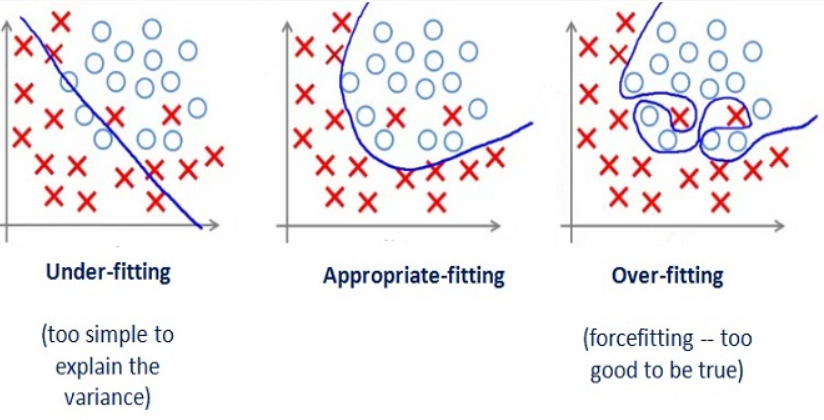
\includegraphics[width=12cm]{Bilder/overUnderfitting.png}
		\caption{Over- und Underfitting}
		\label{fig:overUnderFitting}
	\end{center}
\end{figure}

Die Abbildung \ref{fig:overUnderFitting} zeigt 3 Graphen, die das Problem erläutern. Jeder Graph visualisiert, wie gut das Modell anhand der Trainingsdaten die einzelnen Punkte in 2 Cluster unterteilt.
\\\\
Das Modell ist unter angepasst, wenn wie im linken Graphen das Model zu schlecht mit den Trainingsdaten abgestimmt wurde. Hier wurden zu wenig Punkte richtig abgedeckt und es konnten zu wenige Muster zwischen den Eigenschaften und dem Label erkannt werden. Solche Modelle neigen zu hohen Verzerrungen der Vorhersagen.
\\\\
Der Graph auf der rechten Seite hingegen sagt alle Punkte richtig vorher. Unter dieser Annahme könnte man denken es wäre ein sehr guter Graph. Hier spricht man allerdings von einer Überanpassung, da das Modell zu gut auf die Trainingsdaten abgestimmt ist, und bei Testdaten schlechte Ergebnisse liefern wird. Ein Grund dafür ist, dass alle Punkte mit vorher gesagt werden, auch diese die Grundrauschen oder Outliner sind. Solche Modelle besitzen eine hohe Varianz der Vorhersagen\cite{overUnderfitting}.
\\\\
Ein Beispiel für z.B. Overfitting ist, wenn durch maschinelles Lernen ein System einen Schrank auf einem Bild erkennen soll. Nun werden zu viele Eigenschaften mit erfasst, welche jede Art an Schränken erkennen soll, auch solche die z.B. Autos ähnlich sehen. Daraufhin könnte es passieren, dass das Modell die Trainingsdaten sehr gut erkennt und sobald man anfängt mit realen Daten zu testen, auf welchen auch Autos vorkommen können, könnte das Programm Autos als Schränke erkennen, da das Modell zuvor zu komplex war.
\\\\
Am besten ist somit der mittlere Graph, welcher Outliner und das Grundrauschen ignoriert und eine gute Balance zwischen Verzerrung und Abweichungen besitzt.
\subsection{Ähnlichkeit der Daten}
\label{section:similarData}
\begin{figure}[h]
	\begin{center}
		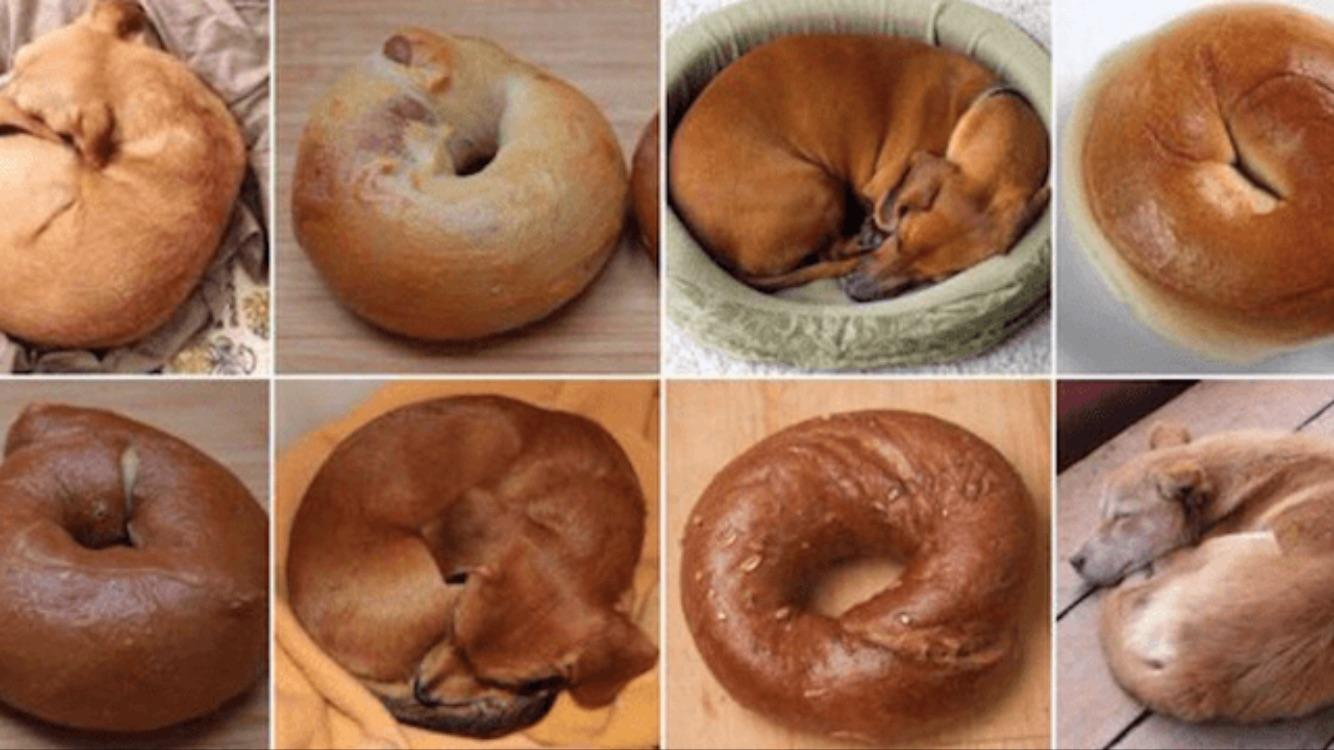
\includegraphics[width=15cm]{Bilder/dog_or_bagel.jpg}
		\caption{Hund oder Bagel?}
		\label{fig:dogBagel}
	\end{center}
\end{figure}

Es gibt optische Täuschungen, die uns etwas anderes wahrnehmen lässt, als eigentlich auf dem Bild zu sehen ist. Anhand des Beispiels aus der Abbildung \ref{fig:dogBagel} wird deutlich, dass wenn die Farbe, Struktur und die Form identisch sind, die Wahrnehmung trüben kann und ein Bagel auf den ersten Blick als Hund identifiziert wird. Dass gilt auch für eine KI, denn eine KI lernt Muster, Strukturen und besondere Eigenschaften anhand der Bilder kennen. Hat man nicht genug Trainingsdaten, um der Maschine diese Unterschiede zu verdeutlichen, kann es hier auch ohne Falsche Eingaben zu einer Verzerrung der Ergebnisse führen.

\section{Menschliche Fehler}
Den Faktor Mensch darf man bei der Bias Entstehung nicht vergessen. Konzeptionelle Fehler mangels an Wissen oder einem Missgeschick heraus fördern Fehlverhalten. Markante Defizite können ein funktionale KI-Entstehung komplett verhindern, sind in der Regel noch die besseren Missstände. Denn kleine Mängel, die nicht sofort auffallen, können in Produktion fatale Folgen haben.
\subsection{Falsche Zielsetzung}
Die Zielsetzung eines KNNs ist ein nicht zu unterschätzender Teil bei der KI Entwicklung. Setzt man hier den falschen Grundstein, können sich vermeidbare Fehlverhalten einer KI entwickelt.
\subsubsection{Subjektive Ziel Definition}
Die Zielvariablen spiegeln die Antworten der Aufgabe wieder, die eine KI lösen soll. Wenn die Frage lautet, findet den besten Mitarbeiter, muss die Zielsetzung in messbare Werte übersetzt werden. Bei dieser Definition kann bewusst oder unbewusst Bias eingepflegt werden. Anhand welcher Werte der 'Beste' Mitarbeiter ist, liegt allein an dem subjektiven Meinung des Entwicklers. Ist die Meinung 'männlich, jung, intelligent' würde die KI Frauen diskriminieren.
% https://www.lernen-wie-maschinen.ai/ki-pedia/was-ist-algorithmische-voreingenommenheit-algorithmic-bias/
\subsubsection{Zu viele Ziele}
Viele Köche verderben den Brei. Diese Weisheit kann auch auf die Ziele von KNNs umgemünzt werden. Denn je mehr Ziele ein KNN hat, desto größer und komplexer muss ein KNN sein, um alle Fälle abdecken zu können. Je komplexer ein KNN ist, desto größer ist die Wahrscheinlichkeit, dass Fehler passieren. Auch ist sich das Netz deutlich unsicherer bei seinen Entscheidungen.
\\\\ % Ohne Quelle :(
Wenn man eine nahezu perfekte KI mit einer Aufgabe erweitern möchte, hat das meist zu Folge, dass die KI nach der Erweiterung zwar mehr kann, jedoch seine ehemalige Hauptaufgabe nicht mehr so gut meistert wie zuvor.
% Beispiel: Baidu Gesichtserkennung (erkennt nur Asiaten)
\subsection{Falsches Lernen}
% Panzer Beispiel von oben, fällt in die Kategorie 'Falsches Lernen' mit ein
% Unvollständigkeit lieber mit dem Beispiel von Gesichtserkennung iPhone nehmen
KI lernt oft einfachste Unterschiede
\\i.	Nicht Unterschied zwischen Auto und Boot sondern Untergrund(Wasser/Land)
\\ii.	Sehr Fehleranfällig z.B. Auto fährt durch flaches Wasser (KI -> Boot)
\\iii. 	Mensch soll Lernprozess kontrollieren, ob KI auf dem richtigen Weg befindet
\subsection{Bewusste Manipulation der Trainingsdaten}
Vorsätzliches Manipulieren von Trainingsdaten provoziert bewusst Fehlverhalten. Bei geschickter Manipulation ist die Betrug in den Datensätzen nicht erkennbar. Auch die KI funktioniert erwartungsgemäß. Nur bei bestimmten Eingaben tritt ein unerwünschtes Verhalten auf. \\\\
Vor allem bei öffentlichen Datensätzen kann man nicht hundertprozentig sicherstellen, dass keine Manipulation an den Daten vorgenommen wurden.

\chapter{Sicherheitsprobleme durch BIAS}

\section{Gefahren für Maschinen}
Computer, die von Computern gesteuert werden, sind heutzutage keine Science Fiction mehr. In der Industrie 4.0 nimmt KI eine große Rolle ein. Somit können Fehlverhalten nicht nur uns Menschen sondern auch Maschinen schaden.
\subsubsection{Kühlung von Rechenzentren}
Seit 2016 setzt Google eine KI zur Optimierung des Kühlungsprozesses ein. Anfangs lieferte die KI nur Konzepte zur Kühlungsoptimierung, welche Mitarbeiter auswerten und einsetzt konnten. Heutzutage nimmt die KI Änderungen autonom an der Kühlung vor. Bis zu 40 Prozent an Energie konnte somit eingespart werden, was sich einerseits aus ökonomischer und als auch auf finanzieller Sicht lohnt.\\
% Der Teil ist rein spekulativ und nicht belegbar
Unterläuft der KI hier ein Fehler, hat dies direkte Folge auf die Langlebigkeit der Computerelemente des Rechenzentrums und kann bis hin zu Brandherden in Gebäuden führen.
\section{Gefahren für Menschen}
In Zukunft werden KIs immer mehr zu unseren Alltag gehören und greifen immer stärker in unseren Leben ein. Dies hat viele Vorteile, jedoch haben sie ebenso Nachteile insbesondere für ärmere Teile der Bevölkerung sowie Minderheiten.
\subsection{Diskriminierung von bestimmten Personengruppen oder Minderheiten}
Einleitungsvariante 1 \\
Alltagsrassismus ist ein Denkschemata größerer sozialen Gruppen, diese ein 'Wir' konstruieren und andere insbesondere Minderheiten kategorisch ausgeschlossen oder andersartig benachteiligen.\\
Dieses Kategorisieren ist eine Hauptfunktion der KI. Dadurch werden schnell bewusst oder unbewusst Diskriminierungen eingepflegt. Was das für Auswirkungen heute schon hat, zeigen folgende Beispiele.
\\\\ Einleitungsvariante 2\\
Durch die \#BlackLivesMatters Bewegung 2020 ist die Forderung nach Gleichberechtigung aktuell wieder omnipräsent. KI könnte hier abhelfen. Denn KIs sind Programme und können somit keine Vorurteile besitzen. Leider ist die Theorie nur eine Halbwahrheit. Natürlich sind Algorithmen von sich aus nicht rassistisch Motiviert, jedoch spiegeln sie diskriminiertes Verhalten aus Daten oder sonstigen Fehlern heraus wider.
\subsubsection{Bewerbung}
Amazon entwickelte 2014 ein Bewertungssystem, wie bereits in \ref{section:biasInTest} beschrieben.
\subsubsection{Alltagsrassismus}

\subsubsection{Rückfallgefahr}
In Amerika werden KIs eingesetzt um Sozialprognosen von Angeklagten und Häftlingen zu erstellen, benachteiligt eindeutig Schwarze. Nachweislich lag die Software doppelt so oft mit den Prognosen zukünftiger Verbrechen von Afroamerikanern falsch im Vergleich zu weißen Angeklagten. Durch schlechte Sozialprognosen haben Angeklagten eine geringe Chance auf frühzeitige Entlassung. Bedeutet, afroamerikanische Straftäter müssen durchschnittlich länger Inhaftieren als Weiße, dank KIs.
\subsection{Lebensgefahr}
Tesla schickt seine Kunden mit einer Beta-KI autonom auf die Straßen.
\section{Angriff auf KI}
Ist eine Künstliche Intelligenz sehr gut trainiert, erzielt sie in ihrem Aufgabebereich überragende Ergebnisse. Doch auch nahezu perfekte KIs sind nicht unfehlbar. Durch methodisch gestaltete Störungen der Eingeben kann eine KI bewusst getäuscht werden und die Computer-Wahrnehmung in die Irre führen. Diese Art der Ausnutzung von KI Schwächen nennt man Adversarial Attacks, zu deutsch gegensätzlicher Angriff.
\subsubsection{Adversarial Attacks}
Bildererkennungssoftware ist besonders anfällig für dieser Art von Angriff. Hierbei legt man über das Bild bestimmte Pixelmuster, die für das menschliche Auge in der Regel im Gesamtbild untergehen. KIs hingegen registrieren jegliches Muster und nehmen sie in ihre Berechnungen mit auf. Als Ergebnis werden Bilder zum Teil massiv fehlinterpretiert.
Im Folgenden Angriff wird mit einer Brille und dessen speziellen Muster, eine KI überlistet.
\label{section:BrilleAttack}
\begin{figure}[h]
	\begin{center}
		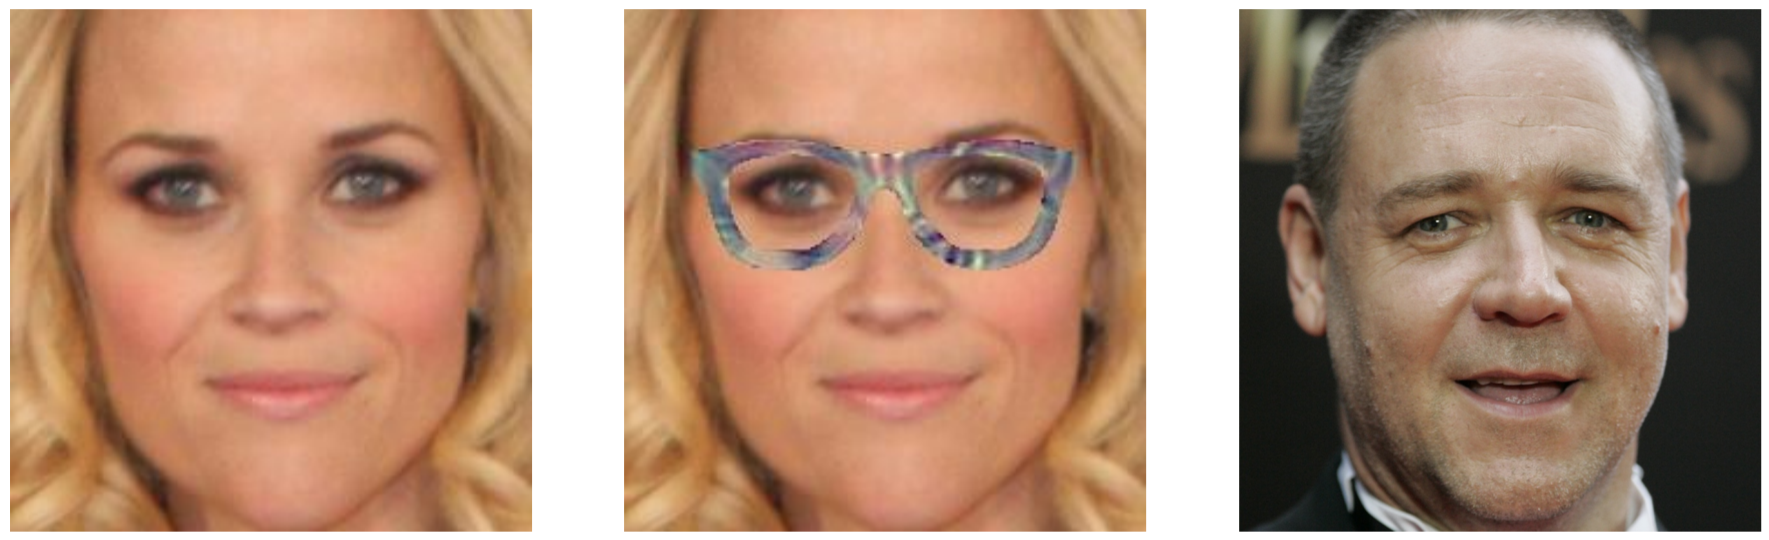
\includegraphics[width=15cm]{Bilder/Brille_Adversarial_Attack.png}
		\caption{Reese Witherspoon links korrekt identifiziert. Mitte Bild mit Adversarial Attack. Rechts Klassifizierung von Mitte als Russel Crowe}
		\label{fig:BrilleAttack}
	\end{center}
\end{figure}
% Paper https://www.cs.cmu.edu/~sbhagava/papers/face-rec-ccs16.pdf
Im linken Bild sieht man die amerikanische Schauspielerin Reese Witherspoon. Dieses Bild wird auch korrekt als sie selbst von der KI erkannt. Setzt man nun ihr eine spezielle Brille auf, beginnt das neuronale Netz Fehler zu begehen. Plötzlich erkennt die KI Reese Witherspoon mit der Brille als Russel Crowe (Bild rechts).

%https://www.inovex.de/blog/machine-perception-face-recognition/
\chapter{Prävention}
\label{chapter:main}
\section{Passender Algorithmus zu Daten}

Im Abschnitt \ref{section:DataGarbage} wurden die Schwierigkeiten genannt, was passiert wenn ein Modell mit fehlerhaften Daten trainiert wurde und ab einem gewissen Grad es schwer wird diese fehlerhaften Vorhersagen zu verstehen und abzuändern.
\\\\
In der Annahme das nun dieses System richtig trainiert wurde, aber die zeitliche Komponente nicht beachtet, wie z.B. dass ein Panzer in Zukunft anders ausschauen könnte, kann es zu dem Problem kommen, das in Zukunft ein Panzer nicht mehr erkannt wird. Wie Stöcker 2019(\cite{stoecker}) bereits erwähnte, benötigt eine sich ändernde Gesellschaft auch kontinuierliche weiterlernende Algorithmen.
\\\\
Solch ein Lernprozess wird auch als \textit{adaptive learning} bezeichnet, womit dem Effekt sich ändernder, d. h. dynamischer Datenumgebungen, concept drift bezeichnet, Rechnung getragen wird \cite{gama}. In DL-Algorithmen ist solche eine Umsetzung nicht trivial, aber das Beispiel von Sahoo et al. \cite{sahoo} zeigt auch die Machbarkeit auch in diesem Feld.
\\\\
Auch bei einem für Diskriminierung anfälligen Umfeld, wie im Beispiel von Abschnitt \ref{section:biasInTest}, muss besondere Sorgfalt bei der Wahl des passenden Algorithmus bedacht werden. Oftmals ist es unzureichend einzelne Attribute aus den Eingangsdaten auszuschließen, um beispielsweise eine algorithmische Diskriminierung bestimmter Personengruppen zu verhindern. Dies genügt jedoch in der Regel nicht, denn wie das Beispiel von Amazon zeigt, kann der Algorithmus Rückschlüsse anhand anderer Attribute ziehen(z.B. durch Frauenvereine).
\\\\
In diesem Kontext sollten System bevorzugt werden, welche in der Entwicklung solcher Algorithmen zusätzliche Einschränkungen einführen, um eine Diskriminierung aufgrund eines bestimmten Attributs, zu verhindern \cite{kamiran}.

\section{Nur ein Ziel}
\label{section:oneGoal}
Nimmt man das Beispiel aus dem Abschnitt \ref{section:OverUnderfitting} mit den Schränken und möchte der Maschine alle möglichen Schränke beibringen, kann dies wie in diesem Absatz bereits erläutert zu Overfitting führen. Das Ziel aus diesem Beispiel war zu komplex. Hier hätte man das Ziel einfacher halten und die Daten generalisieren sollen. Dass heißt sich auf Schränke beschränken die sofort als solche erkannt werden. Falls ein Schrank ein komplizierteres Aussehen hätte und durch den Algorithmus nicht erkannt worden wäre, wäre das besser als wenn der Algorithmus viele Autos als Schränke erkennt.
\\\\
Solche Probleme treten häufig auf, da die Ziele meist zu komplex gehalten werden. Das führt zu einer großen Fehleranfälligkeit und somit zu Verzerrungen. Deswegen sollten die Ziele klar und einfach gehalten werden, um unnötige Komplexität zu vermeiden.

\section{Verfahren zum Validieren}
\label{section:validate}

Damit Vorurteile, Outliner oder falsche Bilder in den Daten nicht zu Problemen führen sollte diese zuvor überprüft werden. Beispiele dafür könnten folgende sein:
\begin{enumerate}
	\item Lektorat oder Peer-Review
	\item Das Vier-Augen-Prinzip (gegenseitige Kontrolle)
	\item Mehrheitsentscheide bei unterschiedlichen Ergebnissen
\end{enumerate}

Zudem sollte das Modell ausreichend validiert werden und die Performance gemessen werden. Denn wenn der Algorithmus z.B. bei der Diagnose von Krebs helfen soll, sollten die Ergebnisse nicht falsch sein.
\\\\
Würde man einen Datensatz in Trainings und Testdaten unterteilen, könnte es dazu kommen, das die Daten so perfekt aufgeteilt werden, dass er in dieser Aufteilung sehr gute Ergebnisse liefert. Falls nun aber ein Fall nur in den Testdaten vorhanden ist und somit nicht antrainiert wurde, jetzt aber in der realen Welt benötigt wurde, können die Ergebnisse trüben und das Modell könnte zu Problemen führen.
\\\\
Eine Möglichkeit um das zu verhindern, bietet die Cross Validierung. Anstelle eines extra Datensatzes, welcher zum Validieren der Daten genutzt wird, wird der Datensatz in viele kleine Blöcke unterteilt. In der Abbildung \ref{fig:crossValidierung} sind es 5. Danach werden 5 Durchläufe gemacht, in denen jeweils mit 4 unterschiedlichen aus diesen 5 Blöcken trainiert und mit einem davon getestet wird. Bei jedem Durchlauf entsteht ein Score, welche angibt, wie gut das Modell ist. Am Ende wird dann ein durchschnittlicher Score über diese 5 einzelnen gebildet, welcher die gesamt Performance des Modells angibt.

\begin{figure}[h]
	\begin{center}
		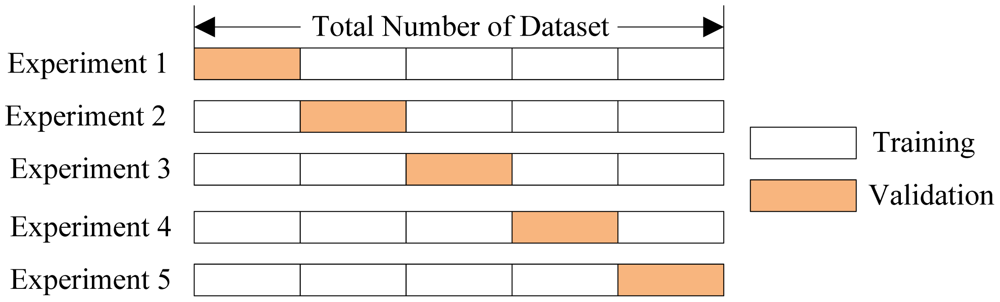
\includegraphics[width=15cm]{Bilder/crossValidierung.png}
		\caption{5 fache Cross Validierung}
		\label{fig:crossValidierung}
	\end{center}
\end{figure}

Mit diesem Score lässt sich das beste Modell ermitteln und man verhindert unbewusste Nebenwirkungen.

\section{Over- und Underfitting vermeiden}
\label{section:preventData}

Underfitting und Overfittung sind oft Fehler der Test-/Trainingsdaten Aufbereitung. Um Overfitting zu verhindern, kann ein einfacheres Ziel wie bereits in Absatz \ref{section:oneGoal} beschrieben, ausreichen. Dennoch gibt es Fälle wo das Ziel zu komplex ist oder zu wenig Daten vorhanden sind, um Underfitting oder Overfitting zu verhindern.

\subsection{Underfitting}

Anhand einer polynominialen Regression kann man verdeutlichen, wie Underfitting vermieden werden könnte. Um dies zu erreichen, muss der erwartete Wert einer Variable als Polynom n-ten Grades modelliert werden, welches dann wiederum das allgemeine Polynom ergibt. Wenn wir den Grad ${n}$ des Polynoms erhöhen, nimmt der Trainingsfehler generell ab. Die allgemeine Gleichung eines Polynoms ist folgende:

${\displaystyle y=\beta_{0}+\beta_{1}x+\beta_{2}x^{2}+...+\beta_{n}^n+\epsilon}$

Aber hier muss aufgepasst werden. Denn wie in der Abbildung \ref{fig:polyReg} zu sehen sinkt zur gleichen Zeit der Cross Validierungsfehler solange wir n bis zu einem gewissen Punkt erhöhen, nach diesem Punkt steigt der Fehler und Overfitting wird das Problem.

\begin{figure}[h]
	\begin{center}
		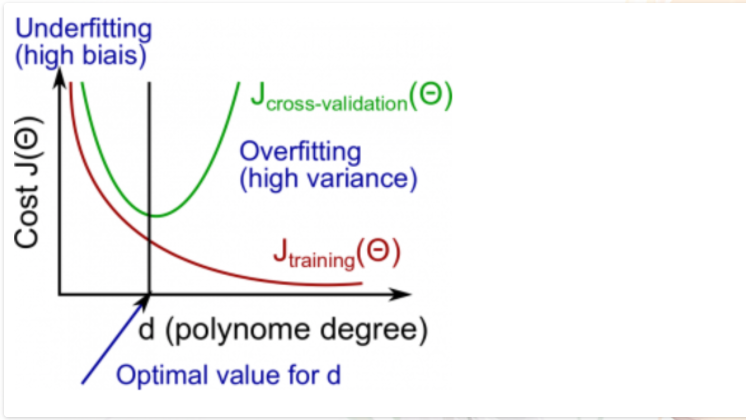
\includegraphics[width=15cm]{Bilder/polynomeRegression.png}
		\caption{Polynominale Regression}
		\label{fig:polyReg}
	\end{center}
\end{figure}

\subsection{Overfitting}

Eine Möglichkeit um Overfitting zu vermeiden bietet die bereits in Abschnitt \ref{section:validate} Cross Validierung. Eine andere kann durch das erhöhen der Flexibilität des Models erreicht werden. Um die Flexibilität zu erhöhen können Regulierungstechniken benutzt werden.
\\\\
Durch die Regulierung wird wenn die Komplexität eines Models zunimmt, eine Strafe angehängt. Der Regulierungsparameter (${\lambda}$) bestraft alle Parameter mit Ausnahme des markierten Bereichs in Abbildung \ref{fig:regFunc}, sodass das Modell die Daten verallgemeinert und nicht überanpasst.

\begin{figure}[h]
	\begin{center}
		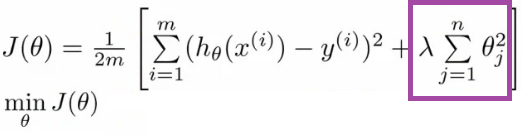
\includegraphics[width=10cm]{Bilder/regFunc.png}
		\caption{Regularisierung in Loss Funktion}
		\label{fig:regFunc}
	\end{center}
\end{figure}

Wenn in der Abbildung \ref{fig:regFunc} die Komplexität steigt, wird durch die Regulierung eine Strafe für höhere Terme hinzugefügt. Dass hat zur Folge, dass die Wichtigkeit solcher langen Terme sinkt und zugleich die Komplexität des Models weniger wird.
\\\\
Beispiele für solche Techniken sind folgende:

\begin{enumerate}
	\item L1 Regulierung (Lasso Regulierung)
	\item L2 Regulierung (Ridge Regulierung)
	\item Elastic net
\end{enumerate}


\chapter{Fazit}
Thema ist größer als hier beschreibbar
\\Evtl. Deep Fake
http://iphome.hhi.de/samek/pdf/LapNCOMM19.pdf
https://ujjwalkarn.me/2016/08/11/intuitive-explanation-convnets/


\backmatter
%%%%%%%%%%%%%%%%%%%
%% create tables list
%%%%%%%%%%%%%%%%%%%
%\listoftables

%%%%%%%%%%%%%%%%%%%
%% create listings list
%%%%%%%%%%%%%%%%%%%
%\lstlistoflistings
%\addcontentsline{toc}{chapter}{Listings}

\cleardoublepage
\phantomsection
\addcontentsline{toc}{chapter}{Literatur}
\printbibliography

\end{document}
